
\documentclass[a4paper,12pt]{article} 
\usepackage{graphicx}
\begin{document}
\title{SCI 101-03 Homework 2}
     \author{Louie Celiberti}
     \date{February 15th 2020}
     \maketitle
     
\section{Career Goal}
After graduating from Manhattan college, I intend to become a software engineer, working for some technology or bank company. Before becoming a software engineer, I will be applying for internships and research oppurtunities throughout my next four years at Manhattan College.

\section{Identification Photo}
\begin{center}
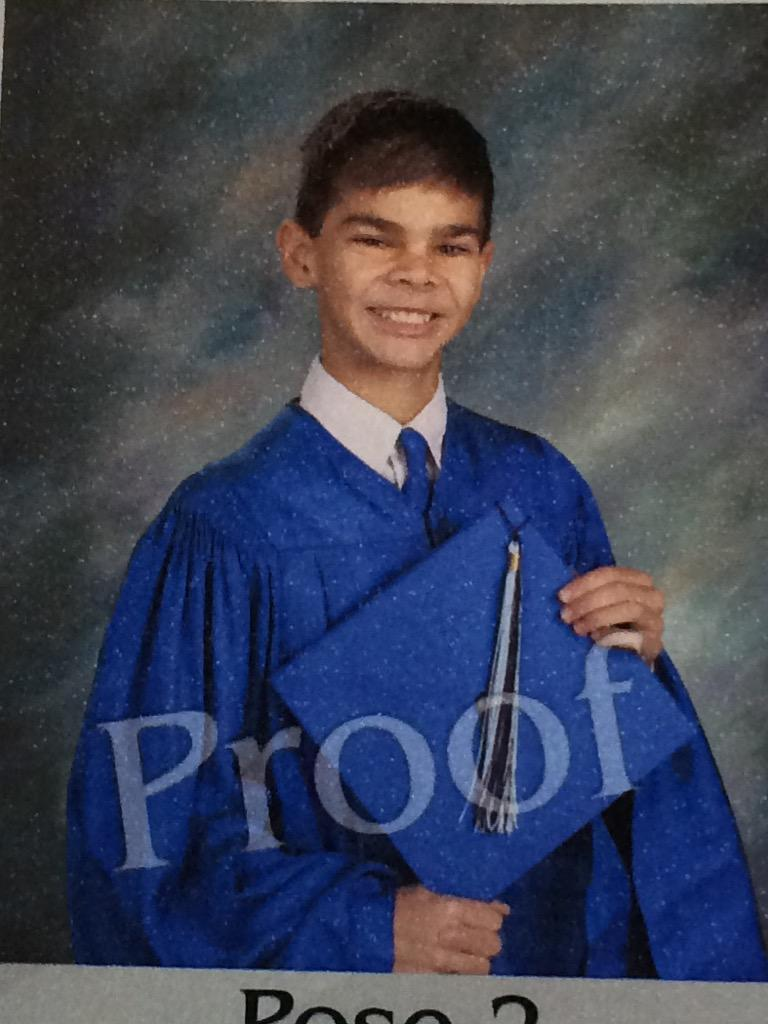
\includegraphics[width= 75mm]{graduation.png}
\end{center}

\section{Multiplication Table}
\begin{center}
\begin{tabular}{ c| c | c | c | c | c | c | c | c | c | }
1& 2 & 3 & 4 & 5 & 6 & 7 & 8 & 9\\
\hline
2& 4 & 6 & 8 & 10 & 12 & 14 & 16 & 18 \\ 
\hline
3& 6 & 9 & 12 & 15 & 18 & 21 & 24 & 27\\ 
\hline
4& 8 & 12 & 16 & 20 & 24 & 28 & 32 & 36\\ 
\hline
5& 10 & 15 & 20 & 25 & 30 & 35 & 40 & 45 \\ 
\hline
6& 12 & 18 & 24 & 30 & 36 & 42 & 48 & 54\\

\hline
7& 14 & 21 & 28 & 35 & 42 & 49 & 56 & 63 \\ 
\hline
8& 16 & 24 & 32 & 40 & 48 & 56 & 64 & 72\\ 
\hline
9& 18 &  27 & 36 & 45 & 54 & 63 & 72 & 81 \\ 
\hline
\end{tabular}
\end{center}

\section {Mathematical Equations}
\begin{center}
\huge$x=\frac{-b\pm\sqrt{b^2-4ac}}{2a}$
\end{center}
\end{document}
